\documentclass[a4j]{jarticle}
\usepackage[dvipdfmx]{graphicx}
\usepackage[dvipdfmx]{color}
\usepackage{url}
\usepackage{here}

\begin{document}



% 成長記録%

\section{成長記録}\label{grow}
図\ref{Grow}に、成長記録起動時の画面を示します。
成長記録は、自分の撮影した子どもの写真やゲームの記録を保存し、閲覧及び共有することができます。

\begin{figure}[H]
    \begin{center}
    \resizebox{8cm}{!}{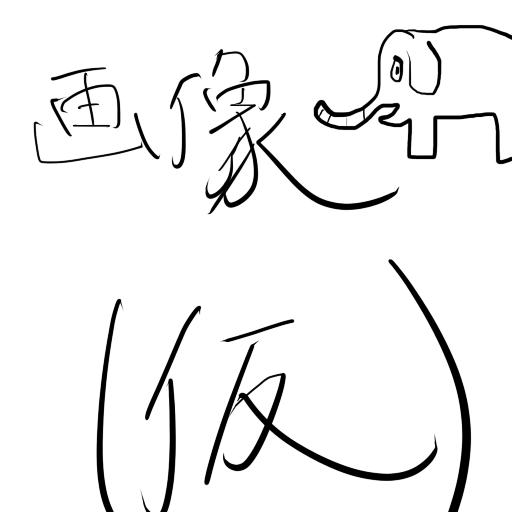
\includegraphics {kari.png}}
    \caption {成長記録の画面}
    \label{Grow}
    \end{center}
\end{figure}

\begin{enumerate}
  \renewcommand{\labelenumi}{\textcircled{\scriptsize \theenumi}}
  \item 写真及びゲーム記録\\
       撮影した写真やゲームの記録を閲覧することができます。各写真や記録をタップすると拡大して表示され、保存は月ごとにされていきます。また、メモを残すこともできます。
  \item カメラボタン\\
        撮影したいときに使用するボタンです。ボタンを押すと外部のカメラアプリを起動し写真を撮影することができます。
  \item 共有ボタン\\
        写真やゲームの記録を共有したい時に使用するボタンです。ボタンを押すと外部アプリ(Twitter)を起動し共有することができます。
\end{enumerate}

\subsubsection{アルバム画面}\label{albam}
図\ref{Albam}に、写真をタップしたときの画像を示します。
写真や記録は拡大して表示されます。また、共有ボタンもありここから外部アプリ(Twitter)を起動し共有することができます。

\begin{figure}[H]
    \begin{center}
    \resizebox{8cm}{!}{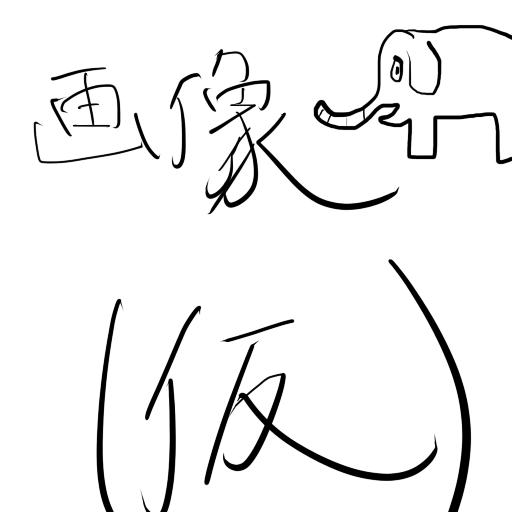
\includegraphics {kari.png}}
    \caption {アルバム画面}
    \label{Albam}
    \end{center}
\end{figure}

アルバムに保存された写真や記録にはコメントボタンを押すことによりコメントを残すことができます。\ref{Comment}にコメント入力の画面を示します。

\begin{figure}[H]
    \begin{center}
    \resizebox{8cm}{!}{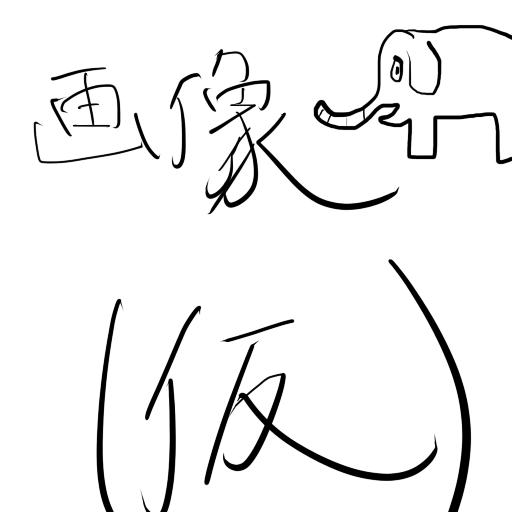
\includegraphics {kari.png}}
    \caption {コメント入力画面}
    \label{Comment}
    \end{center}
\end{figure}


\subsubsection{カメラ}
図\ref{camera}に、カメラ起動時の画面を示します。
カメラを使用して撮影するときに使用されます。カメラは外部アプリとなっており、ここで撮影された写真はアルバムとして保存され\ref{albam}のように閲覧、共有することができます。


\begin{figure}[H]
    \begin{center}
    \resizebox{8cm}{!}{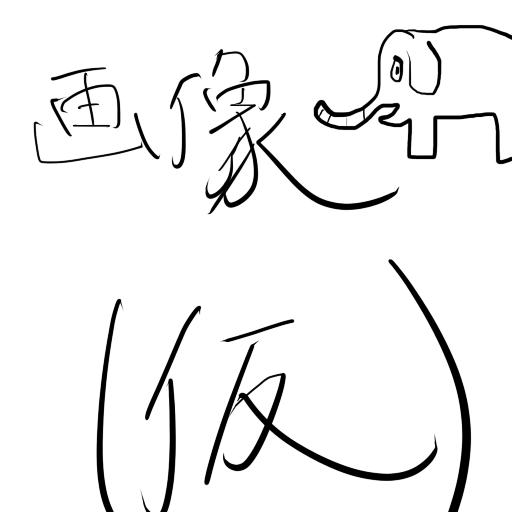
\includegraphics {kari.png}}
    \caption {カメラ画面}
    \label{Camera}
    \end{center}
\end{figure}


\subsubsection{共有}
図\ref{share}に、共有画面を示します。
写真や記録を他社に共有したいときに使用されます。共有は外部アプリであるTwitterで行われます。共有するためには\ref{grow}と\ref{albam}についている共有ボタンを押すことで起動することができます。

\end{document}